\documentclass{article}
\usepackage[utf8]{inputenc}
\usepackage{tikz}
\usepackage{pgfplots}
\usetikzlibrary{shapes.geometric, arrows}

\tikzstyle{startstop} = [rectangle, rounded corners, minimum width=3cm, minimum height=1cm,text centered, draw=black, fill=green!30]

\tikzstyle{io} = [circle, minimum width=1cm, minimum height=1cm, text centered, text width=1cm, draw=black, fill=blue!30] 

\tikzstyle{process} = [rectangle, minimum width=3cm, minimum height=1cm, text centered, text width=3cm, draw=black, fill=orange!30]

\tikzstyle{decision} = [diamond, minimum width=3cm, minimum height=1cm, text centered, draw=black, fill=green!30]

\tikzstyle{arrow} = [thick,->,>=stealth]

% for the legend
% argument #1: any options
\newenvironment{customlegend}[1][]{%
    \begingroup
    % inits/clears the lists (which might be populated from previous
    % axes):
    \csname pgfplots@init@cleared@structures\endcsname
    \pgfplotsset{#1}%
}{%
    % draws the legend:
    \csname pgfplots@createlegend\endcsname
    \endgroup
}%

% makes \addlegendimage available (typically only available within an
% axis environment):
\def\addlegendimage{\csname pgfplots@addlegendimage\endcsname}


\begin{document}

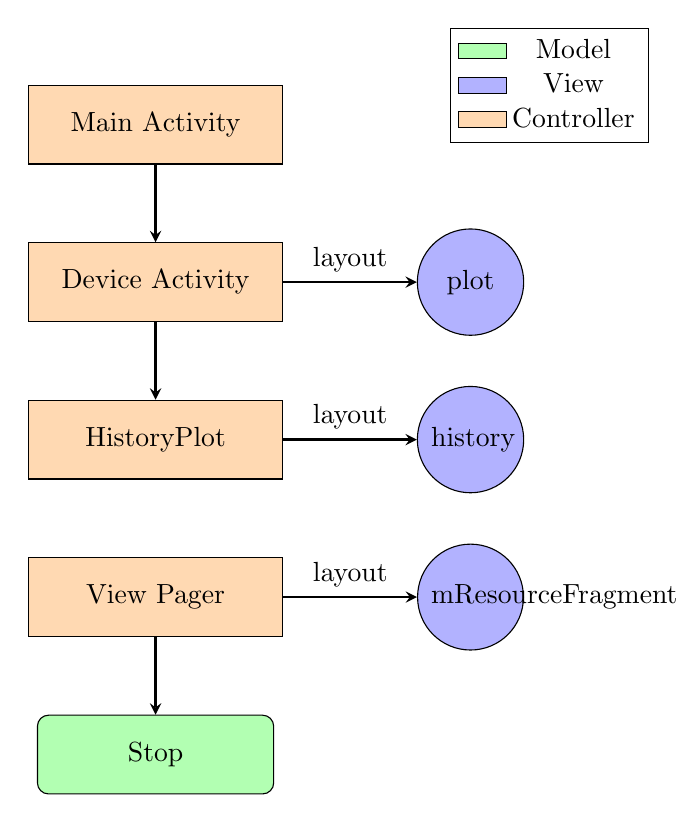
\begin{tikzpicture}[node distance=2cm]

\node (main) [process] {Main Activity};

\node (da) [process, below of=main] {Device Activity};
\node (plot) [io, right of=da, xshift=2cm] {plot};

\node (hist) [process, below of=da] {HistoryPlot};
\node (history) [io, right of=hist, xshift=2cm] {history};

\node (VPA) [process, below of=hist] {View Pager};
\node (fragpage) [io, right of=VPA, xshift=2cm] {mResourceFragmentPager};
\draw [arrow] (VPA) -- node[anchor=south] {layout} (fragpage);

\node (stop) [startstop, below of=VPA] {Stop};

\draw [arrow] (main) -- (da);
\draw [arrow] (da) -- (hist);
\draw [arrow] (da) -- node[anchor=south] {layout} (plot);
\draw [arrow] (hist) -- node[anchor=south] {layout} (history);
\draw [arrow] (VPA) -- (stop);


%%% second legend
%%% http://tex.stackexchange.com/questions/54794/using-a-pgfplots-style-legend-in-a-plain-old-tikzpicture 

\begin{customlegend}[legend entries={Model,View,Controller}, legend style={at={(5,0.5)},anchor=center}]
  \addlegendimage{black,fill=green!30,area legend}
  \addlegendimage{black,fill=blue!30,area legend}
  \addlegendimage{black,fill=orange!30,area legend}
\end{customlegend}

\end{tikzpicture}

\end{document}